O uso efetivo do aprendizado ativo depende de escolhas adequadas diante da diversidade existente de estratégias e de algoritmos de aprendizado de máquina.
Nesta tese, são empreendidas investigações em três níveis sobre esse problema:

\begin{itemize}
\item análise comparativa de estratégias de amostragem ativa;
\item controle da influência do aprendiz durante o processo de amostragem ativa; e,
\item recomendação automática de estratégias.
\end{itemize}

%análise comparativa de estratégias; controle da influência do algoritmo de 
% vou dar nome aos bois na próxima frase
%aprendizado de máquina durante a rotulação; e, emprego de recomendação automática de estratégias.
O primeiro nível de investigação é essencialmente qualitativo e será apresentado por meio de experimentos no Capítulo \ref{experimentos}.
Os dois últimos níveis resultaram na proposta de duas abordagens automáticas, 
respectivamente:  
 estratégia híbrida baseada na inibição do aprendiz
%  enquanto ele for potencialmente prejudicial
- apresentada na Seção \ref{newstrats} juntamente com sua versão puramente agnóstica (Seção \ref{estag}); e, aprendizado meta-ativo - apresentado na Seção \ref{sec:ama}.
A Seção \ref{newstrats} também contém a proposta de adaptação da estratégia SG-\textit{network} a problemas com mais de duas classes.

\section{Estratégias}\label{newstrats}
Em certos casos, o problema da escolha do algoritmo de aprendizado mencionado previamente na Seção \ref{ea} pode ser contornado pela adoção de uma estratégia sem aprendiz.
Uma aplicação hipotética seria o treinamento de um sistema de reconhecimento de conteúdo impróprio, onde o especialista em aprendizado de máquina estivesse interessado em disponibilizar ao público somente conteúdos que tenham sido aprovados previamente por modelos preditivos suficientemente treinados.
Nesse caso, apenas o modelo final é de interesse.
Logo, pode-se empregar uma estratégia sem aprendiz, como a baseada em densidade proposta a seguir, na Seção \ref{newag}.
No contexto desta tese, sua finalidade é facilitar a identificação do efeito da ausência de aprendiz.

Por outro lado, a presença do aprendiz durante o aprendizado pode ser útil mesmo em aplicações que o dispensem.
Na Seção \ref{newhtu}, uma estratégia híbrida, que alterna períodos de presença e ausência de aprendiz, é proposta.

\subsection{Ponderada por densidade sem aprendiz}\label{newag}
Resumidamente, a estratégia TU (baseada em densidade e \textit{Training Utility} - Seção \ref{dw}) pondera a medida de informatividade $\info$ de cada exemplo, afastando a possibilidade de consulta daqueles próximos aos já rotulados e aumentando as chances daqueles situados nas regiões com maior concentração de exemplos não rotulados - conforme depreende-se das equações \ref{eqid} e \ref{eqtu}.
Esse efeito é mais forte quando a densidade é muito alta, pois ela tende a ser a componente dominante da densidade de informação $\stratID$.
Isso faz com que $\info$ tenda a perder relevância.

Dado que a medida $\info$ já é explorada isoladamente pela estratégia Mar (baseada em incerteza - Seção \ref{estsunc}), resta a possibilidade de exploração isolada da parte referente à densidade. 
Assim, a fórmula da função-critério de consulta da nova estratégia \cite{bracis15}, chamada \ing{\sigla{ATU}{amostragem agnóstica ponderada por densidade}}{density-weighted Agnostic sampling (Training Utility)} é apresentada na Equação \ref{eq:agtu}.
\begin{equation}\label{eq:agtu}
 \stratIDATU(\bm{x}) =
 \left(
 \frac{1}{|\mathcal{U}|}
 \sum_{\bm{u} \in \mathcal{U}} sim(\bm{x},\bm{u})
 \right)^\alpha
 \left(
 \frac{1}{|\mathcal{L}|}
 \sum_{\bm{l} \in \mathcal{L}} sim(\bm{x},\bm{l})\right)^{-\delta}
\end{equation}
Onde os parâmetros $\alpha$ e $\delta$ mantêm os significados dados na definição de TU.
Ela é chamada \textit{agnóstica} com base no uso original do termo, que propõe chamar agnóstico o aprendizado que não faz suposições sobre a distribuição dos dados\footnote{\citeonline{conf/isaim/DasguptaHM08} apresentam outro ponto de vista, definindo como \textit{aprendiz ativo agnóstico} aquele que não assume a existência de uma fronteira de decisão perfeita.} \cite{journals/ml/KearnsSS94}.
Seu funcionamento segue o Algoritmo \ref{algo}, geral, apresentado previamente no Capítulo \ref{contexto}, onde a função-critério passa a ser definida da seguinte forma: $q=\stratIDATU$.
% an agnostic active learner (one that does not assume a perfect separator exists)
% http://machinelearning.wustl.edu/mlpapers/paper_files/NIPS2007_178.pdf
% o cenário de aprendizado agnóstico não faz suposições a respeito da origem dos rótulos.
% This is often referred to as the agnostic learning setting,
% since we make no assumptions about the origin of the labels.
% http://www.jennwv.com/courses/F11/lecture4.pdf

Conforme já mencionado, uma vantagem de ATU com relação à maioria das estratégias, é a possibilidade de adiamento da escolha do algoritmo de aprendizado em aplicações que dispensem a disponibilidade do modelo preditivo durante o aprendizado.
Em determinadas situações, também pode ser útil a possibilidade de conhecer toda a sequência de consultas antes de qualquer interação com o oráculo.
Como, frequentemente, o limite de consultas é uma quantidade conhecida de antemão \cite{settles2010active}, elas podem ser repartidas entre vários oráculos que podem trabalhar de forma independente entre si.
Diferentemente, essa possibilidade de paralelização não existe plenamente, por exemplo, na estratégia HS (baseada em agrupamento hierárquico - Seção \ref{estag}).
Mesmo sem aprendiz, esta é dependente da revelação dos rótulos reais para ser capaz de determinar a pureza de cada grupo na hierarquia.
Outra vantagem de ATU, partilhada por poucas estratégias, como Rnd (amostragem aleatória - Seção \ref{estag}), é a inexistência de tempo de espera entre as consultas.

\subsection{Híbrida ponderada por densidade}\label{newhtu}
\simbolo{\rho}{correlação de Pearson entre medidas de Mar e TU}
\simbolo{\rho_{\limiar}}{valor limite para $\rho$}
A abordagem sem aprendiz baseada em densidade (ATU - Seção \ref{newag}) é de natureza exploratória, pois enfoca as regiões mais desconhecidas (sem rótulos) do espaço de exemplos.
Devido à ausência de aprendiz, não há uma fronteira de decisão a considerar.
Logo, não é possível realizar consultas de caráter prospectivo que ataquem diretamente os exemplos mais críticos de forma análoga a uma busca binária.
Entretanto, ambas abordagens, prospectiva e exploratória, têm limitações.
Se, por um lado, a premissa de fronteira única ou perfeitamente separável de uma busca binária não pode ser garantida;
por outro lado, a amostragem puramente exploratória pode ser dispendiosa, pois se assemelha a uma busca exaustiva.
Assim, é intuitivo supor que o equilíbrio entre exploração e prospecção possa vir a ser proveitoso.
A estratégia TU, por exemplo, combina ambas as abordagens em sua fórmula, mas não permite que elas ajam separadamente.

A Figura \ref{domina} ilustra, para o conjunto de dados \textit{Banana} \cite{bache2013uci}, a evolução da função-critério de TU e suas respectivas componentes de exploração e prospecção, correspondentes às estratégias ATU e Mar, respectivamente.
As curvas ATU e Mar são constituídas pelos valores que essas estratégias atribuiriam ao exemplo selecionado por TU.
Os modelos foram gerados pelo algoritmo \textit{Naive Bayes} \cite{conf/ecml/Lewis98}.
\begin{figure}
	\centering
	\includestandalone[mode=buildmissing]{prop1}
	\caption[Curvas das funções-critério para os exemplos selecionados por TU.]{Curvas de valores das funções-critério para os exemplos selecionados por TU.}
	\label{domina}
\end{figure}
Nota-se uma alta correspondência entre as curvas Mar e TU, especialmente nas primeiras 50 consultas.
Essa dominância da componente Mar na determinação da função-critério TU impede que a característica exploratória de ATU influencie significativamente na escolha dos exemplos.
A curva da componente ATU é descendente, indicando a progressiva redução de áreas desconhecidas no espaço de exemplos, porém com oscilações devido à ordem imposta por TU às consultas.

Caso os exemplos fossem escolhidos de acordo com o critério de ATU, as curvas seriam como aquelas apresentadas na Figura \ref{domina2}.
A curva ATU é monotônica descendente conforme esperado, pois cada exemplo consultado (e retirado da reserva) tem o valor de densidade mais alto naquele momento.
Em divergência com a curva da componente Mar na figura anterior, o aprendiz se manteve na região de incerteza por mais tempo e atingiu valores acima de $0,9$ em quase todas as 140 primeiras consultas.
Pode-se supor que essa maior incidência de exemplos incertos se deva à descoberta antecipada de novos segmentos da fronteira de decisão em regiões que permaneceriam inexploradas caso a incerteza do aprendiz (componente Mar) influenciasse as consultas.
Assim, apesar de ser um resultado para um conjunto de dados específico, existe a possibilidade de que outros conjuntos possam se beneficiar desse potencial de antecipação da consulta de exemplos da parte desconhecida da fronteira.
\begin{figure}
	\centering
	\includestandalone[mode=buildmissing]{prop2}
	\caption[Curvas das funções-critério para os exemplos selecionados por ATU.]{Curvas de valores das funções-critério para os exemplos selecionados por ATU.}
	\label{domina2}
\end{figure}

Propõe-se, aqui, uma nova estratégia \cite{bracis15} - chamada \ing{\sigla{HTU}{amostragem híbrida ponderada por densidade}}{Density-weighted Hybrid Sampling (Training Utility)}.
Ela procura alternar as estratégias TU e ATU de acordo com o nível de contribuição corrente da componente exploratória em TU.
O nível de contribuição é estimado por meio do cálculo da correlação de Pearson $\rho$ \cite{books/daglib/0000786} entre as funções-critério de TU e sua componente não-agnóstica (Mar) para toda a reserva de exemplos.
% Evans:
%          .00-.19 “very weak”
%          .20-.39 “weak”
%          .40-.59 “moderate”
%          .60-.79 “strong”
%          .80-1.0 “very strong”
Um valor acima de 0,8, ou seja, representando uma correlação \textit{muito forte} de acordo com \citeonline{evans1996straightforward}, indica uma baixa contribuição da componente exploratória.
Outra interpretação é que, havendo baixa correlação entre os níveis de relevância atribuídos aos exemplos, o aprendiz esteja interferindo excessivamente no critério de consulta - possivelmente por estar ainda no estágio inicial do aprendizado e ser incapaz de realizar predições estáveis ou confiáveis.
Ainda outra interpretação, mais intuitiva, é que a exploração (ATU) prossegue até que as consultas se aproximem tanto da fronteira a ponto de serem similares aos exemplos mais incertos, isto é, consultas similares àquelas que seriam feitas por TU.
A partir desse ponto, ou enquanto a correlação se mantivesse elevada, poder-se-ia considerar que a etapa de exploração não é mais necessária.
Isso é observável na Figura \ref{domina3}, resultante da sequência de consultas gerada por HTU.
\begin{figure}
	\centering
	\includestandalone[mode=buildmissing]{prop2b}
	\caption[Curvas das funções-critério para os exemplos selecionados por HTU.]{Curvas de valores das funções-critério para os exemplos selecionados por HTU.}
	\label{domina3}
\end{figure}
Exceto pela mesma brusca oscilação inicial, provavelmente devido aos primeiros segmentos de fronteira descobertos, a situação é, de certa forma, invertida com relação à situação da Figura \ref{domina}: Mar e TU passam a coincidir na segunda metade do gráfico e o nível de incerteza se mantém elevado.
Como resultado, Mar apresenta a curva mais elevada dentre as três figuras.
Isso indica que exemplos mais incertos e mais informativos\footnote{A única diferença entre HTU e TU é a possibilidade de ausência de aprendiz da primeira.
Consequentemente, se todos os segmentos de fronteira já estivessem revelados, os valores de incerteza apresentados por TU seriam o limite teórico para os valores de incerteza apresentados por HTU (e ATU).
Logo, a elevação que HTU causou nos valores de incerteza se dá devido ao descobrimento de novos segmentos de fronteira.
Trata-se, portanto, de exemplos mais informativos.} foram consultados.

O valor limite de correlação $\rho_{\limiar}$ escolhido para os experimentos deste documento, inclusive o descrito anteriormente, foi 0,999.
Esse valor foi definido conforme explicado a seguir.
Um subconjunto de 1000 exemplos foi extraído aleatoriamente de cada conjunto de dados pertencente a um grupo de 12 conjuntos que não foram empregados na fase experimental da presente pesquisa:
\textit{multiple-features, appendicitis, micro-mass-pure-spectra, hayes-roth, cnae-9, breast-tissue-4class, qualitative-bankruptcy, fertility-diagnosis, acute-inflammations-urinary, digits2, lsvt-voice-rehabilitation} e \textit{micro-mass-mixed-spectra} \cite{bache2013uci}.
O valor médio do índice kappa (para problemas multiclasse - \cite{fleiss2013statistical,conf/pkdd/Shah11})
 %,journals/coling/EugenioG04} 
foi adotado como indicador de desempenho numa validação cruzada em 10 partes.
O intervalo de confiança, consequentemente, é dado para $p=0,05$ e $n=120$.
Ele é dado pela Equação \ref{kappa} em função da matriz de confusão $R$ após 100 consultas - onde $e_i(R)$ e $p_i(R)$ são as componentes dos vetores de classes esperadas e preditas de acordo com $R$, respectivamente (Seção \ref{defpro}).
O algoritmo empregado foi o \textit{Random Forest} com 10 árvores \cite{journals/ml/Breiman01}.
% - detalhes metodológicos são apresentados no Capítulo \ref{metodologia}.
\simbolo{\kappa}{índice kappa multiclasse}
\begin{equation} \label{kappa}
\kappa(R) = \left(r(R) - \frac{p_i(R) \cdot e_i(R)}{\sum\limits_{1\leq i \leq |Y|}e_i(R)}\right)\left(1 - \frac{p_i(R) \cdot e_i(R)}{\sum\limits_{1\leq i \leq |Y|}e_i(R)}\right)^{-1}
\end{equation}
A Figura \ref{hist} contém a colocação média para valores de $\rho_{\limiar}$ em diferentes valores e ordens de magnitude no intervalo $[-0,999999; 0,999999]$.
\begin{figure}
	\centering
	\includestandalone[mode=buildmissing]{prop3}
	\caption[Colocação média para diferentes limites de correlação.]{Colocação média para diferentes limites de correlação. O intervalo de confiança é dado para $p=0,05$ e $n=120$.}
	\label{hist}
\end{figure}
Os valores de colocação se encontram entre 8 e 12, sendo 8,46 a melhor.
Assim, optou-se nesta tese pela sua correlação correspondente, $\rho_{\limiar} = 0,999$.
O autor desta pesquisa não considera esse valor crítico.
Ele foi adotado como prova de conceito para o estudo do efeito do controle da presença do aprendiz na curva de aprendizado e no desempenho preditivo.
% Finally, a disadvantage of HTU is its intrinsic need of a learner
% and the corresponding training time,
% incurring in additional computational costs when compared to ATU.
% This can be relevant in applications where the querying time is 
% critical.

A estratégia HTU é descrita pelo Algoritmo \ref{algohtu}.
O efeito esperado é que ela iniba o aprendiz nos períodos em que a influência dele possa ser negativa.
Esse período de inibição pode se estender por todo o aprendizado, no caso de algoritmos que gerem modelos impróprios para prospecção ou mesmo completamente inadequados para o dado problema.
\begin{algoritmo}
\caption{Estratégia híbrida ponderada por densidade.}
\label{algohtu}
\small
\Entrada{
%  \\ $\mathcal{U}$ - pool
%  \\ $\mathcal{L}$ - initial labelled instances
%  \\ $\cent$ - budget (number of labels to acquire)
%  \\ $\rho_{\limiar}$ - Pearson correlation between Mar and TU
 \\ $\mathcal{U}$ - reserva de exemplos
 \\ $\mathcal{L}$ - conjunto inicial de exemplos rotulados
 \\ $\cent$ - orçamento (quantidade de exemplos a rotular)
 \\ $\rho_{\limiar}$ - limite de correlação entre medidas de Mar e TU
}
\Resultado{
%  \\ $\mathcal{L}'$ - final labelled instances
 \\ $\mathcal{L}'$ - conjunto final de exemplos rotulados
}
% \algalging{\htu{$\mathcal{U}$, $\mathcal{L}$, $\cent$}}{
\algalg{\htu{$\mathcal{U}$, $\mathcal{L}$, $\cent$}}{
 \Se{$\cent = 0$}{
%  \If{$\cent = 0$}{
%   \Return $\mathcal{L}$
  \Retorna $\mathcal{L}$
 }
 \Senao{
%  \Else{
  $\theta = \phi(\mathcal{L})$ \\
  $\mu_{M_\theta}=\frac{1}{|\mathcal{U}|} \sum\limits_{\bm{x} \in \mathcal{U}} M_\theta(\bm{x})$ \\
  $\sigma_{M_\theta}=\frac{1}{|\mathcal{U}|} \sum\limits_{\bm{x} \in \mathcal{U}}(M_\theta(\bm{x}) - \mu_{M})^2$ \\
  $\mu_{\stratIDTU}=\frac{1}{|\mathcal{U}|} \sum\limits_{\bm{x} \in \mathcal{U}} \stratIDTU(\bm{x})$ \\
  $\sigma_{\stratIDTU}=\frac{1}{|\mathcal{U}|} \sum\limits_{\bm{x} \in \mathcal{U}}(\stratIDTU(\bm{x}) - \mu_{\stratIDTU})^2$ \\
%   $\rho = (\sigma_{M}^2\cdot\sigma_{\stratIDTU}^2)^{-\frac{1}{2}} \sum\limits_{\bm{x} \in \mathcal{U}} (M_\theta(\bm{x}) - \mu_{M})(\stratIDTU_\theta(\bm{x}) - \mu_{\stratIDTU})$ \come{correlation Mar-TU}\\
  $\rho = (\sigma_{M_\theta}^2\cdot\sigma_{\stratIDTU}^2)^{-\frac{1}{2}} \sum\limits_{\bm{x} \in \mathcal{U}} (M_\theta(\bm{x}) - \mu_{M_\theta})(\stratIDTU(\bm{x}) - \mu_{\stratIDTU})$ \come{correlação Mar-TU}\\
  \Se{$\rho < \rho_{\limiar}$}{  
%   \If{$\rho < \rho_{\limiar}$}{  
   $\bm{\hat{x}} \leftarrow \argmax\limits_{\bm{x}}[\stratIDATU(\bm{x})]$ \\
  }
  \Senao {
%   \Else {
   $\bm{\hat{x}} \leftarrow \argmax\limits_{\bm{x}}[\stratIDTU(\bm{x})]$ \\
  }
  $\mathcal{L}' \leftarrow \mathcal{L} \cup \{\langle \bm{\hat{x}}, o(\bm{\hat{x}}) \rangle\}$ \\
  $\mathcal{U}' \leftarrow \mathcal{U} \setminus \{\bm{\hat{x}}\}$ \\
  \Retorna \htu{$\mathcal{U}'$,$\mathcal{L}'$, $\cent-1$}
%   \Return \htu{$\mathcal{U}'$,$\mathcal{L}'$, $\cent-1$}
}}
\end{algoritmo}

Além das duas estratégias propostas, algumas estratégias precisaram ser adaptadas para problemas multiclasse.
Essas adaptações são apresentadas na Seção \ref{adapmulti}.

\subsection{Adaptações multiclasse}\label{adapmulti}
Algumas estratégias citadas previamente no Capítulo \ref{contexto} são originalmente voltadas a problemas binários.
Por esse motivo, adaptações precisaram ser feitas para que o conjunto de estratégias pudesse ser aplicado a conjuntos de dados com mais de duas classes.

\subsubsection{Busca no espaço de hipóteses multiclasse}
\simbolo{\unidist(i,j)}{distribuição uniforme no intervalo $[i; j] \cap \mathbb{Z}$}
\simbolo{c}{classe negativa}
Conforme explicado na Seção \ref{sgnet}, é possível fazer uma amostragem ativa dentro da perspectiva do espaço de hipóteses.
Uma adaptação chamada \textit{SGmulti} foi proposta para contornar a limitação de aplicabilidade da abordagem original apenas a problemas binários \cite{conf/hais/SantosC14}.
A abordagem original (SG-\textit{network}) depende da existência de uma única classe \textit{positiva}.
São definidos um modelo mais geral $\theta_{G}$ e um modelo mais específico $\theta_{S}$.
Cada modelo simula a especificidade ou a generalidade.
A simulação se dá por meio de exemplos de fundo artificiais da classe oposta \cite{series/synthesis/2012Settles}.

Na presente proposta de adaptação, a existência de mais de duas classes exige mais que dois modelos.
Cada classe $c \in Y$ tem um modelo associado $\theta_c$, onde $c$ corresponde à classe negativa.
O conjunto $Y \setminus \{c\}$ corresponde ao que poderia ser chamado conjunto de ``classes positivas''.
Cada modelo $\theta_c$ é induzido com um conjunto de exemplos ponderados $\mathcal{\bar{L}}_c$, especificado na Equação \ref{lpond}.
\simbolo{\mathfrak{\bar{L}}}{grupo de conjuntos de dados ponderados e artificialmente rotulados}
\begin{equation}\label{lpond}
\mathcal{\bar{L}}_c = \mathcal{\bar{L}} \cup \{\langle \bm{x},c,w \rangle \mid  \bm{x}\in \mathcal{U}, w=(|Y||\mathcal{U}|)^{-1}\}
\end{equation}
Resumidamente, a equação define cada conjunto $\mathcal{\bar{L}}_c$ como $\mathcal{\bar{L}}$ acrescido dos exemplos de $\mathcal{U}$ artificialmente rotulados com a classe $c$.
Tais exemplos são ditos artificiais porque a classe é fictícia, ou seja, não é dada por um rótulo atribuído pelo oráculo.
Tais exemplos são incorporados ao conjunto com um peso $w$ diminuto ($w << 1$), conforme sugerido recentemente na literatura \citeonline{series/synthesis/2012Settles}.
O valor exato de $w$ foi definido de forma que a contribuição de todos os exemplos artificiais nunca superasse a contribuição de um único exemplo real: $\sum\limits_{c \in Y}|\mathcal{\bar{L}}_c \setminus \mathcal{\bar{L}}| = 1$. 
Essa medida evita que os exemplos de fundo se sobreponham aos exemplos reais no início do processo de rotulação.
Essa não sobreposição é importante porque, no início, os exemplos reais rotulados são escassos.

O conjunto $\mathfrak{\bar{L}}$ de todos os conjuntos $\mathcal{\bar{L}}_c$ é definido pela Equação \ref{lspond}.
\begin{equation}\label{lspond}
\mathfrak{\bar{L}} = \{\mathcal{\bar{L}}_c \mid c \in Y\}
\end{equation}

A função de predição $\hat{y}_{\theta}$ retorna a classe mais provável de um dado exemplo $\bm{x}$ de acordo com o modelo $\theta_c$.
É possível encontrar um exemplo $\bm{\hat{x}}$ para o qual não haja consenso comparando os retornos de todas as diferentes funções de predição.
A sequência\footnote{Sequências são mais convenientes que conjuntos para a descrição do procedimento no Algoritmo \ref{algosgm}.} $D$ de exemplos em desacordo é dada pela Equação \ref{eqconctrov}.
\begin{equation}\label{eqconctrov}
D = \langle\bm{x} \in \mathcal{U} \mid c,d \in Y, \hat{y}_{\theta_c}(\bm{x}) \neq \hat{y}_{\theta_d}(\bm{x})\rangle
\end{equation}
Exemplos da região de desacordo ($\bm{\hat{x}} \in D$) são consultados um a um.
Após cada consulta, seu exemplo de fundo correspondente em todos os conjuntos de treinamento recebe o rótulo verdadeiro e peso integral, gerando os novos conjuntos $\mathcal{\bar{L}}_c', c \in Y$ - conforme a Equação \ref{eqsgcon}.
\begin{equation}\label{eqsgcon}
\mathcal{\bar{L}}_c' = (\mathcal{\bar{L}}_c \setminus \{\langle\bm{\hat{x}},c,w\rangle\}) \cup
\{\langle\bm{\hat{x}},o(\bm{\hat{x}}),1\rangle\}
\end{equation}
Depois de cada consulta, os modelos $\theta_c$ são atualizados com os novos conjuntos $\mathcal{\bar{L}}_c', c \in Y$.
Dado o peso diminuto do exemplo artificial que foi substituído, essa atualização equivale a um treinamento incremental apenas com o exemplo $\langle\bm{\hat{x}},o(\bm{\hat{x}}),1\rangle$ - resultando numa ordem de complexidade de $\mathcal{O}(|Y|)$, pois requer treinamento em $|Y|$ exemplos por consulta, um para cada modelo.

Por fim, a estratégia SGmulti é descrita pelo Algoritmo \ref{algosgm}.
\begin{algoritmo}
\caption{Estratégia SGmulti.}
\label{algosgm}
\small
\Entrada{
 \\ $\mathfrak{\bar{L}}$ - conjunto dos conjuntos rotulados (parcialmente) artificiais
 \\ $\cent$ - orçamento (quantidade de exemplos a rotular)
}
\Resultado{
 \\ $\mathcal{L}'$ - conjunto final de exemplos rotulados
}
\algalg{\sgmulti{$\mathcal{U}$, $\mathfrak{\bar{L}}$, $\cent$}}{
  \Se{$\cent = 0$}{
   \Retorna $\mathfrak{\bar{L}}$
  }
  \Senao{
  $\{\mathcal{\bar{L}}_1, \mathcal{\bar{L}}_2, ..., \mathcal{\bar{L}}_{|Y|}\} = \mathfrak{\bar{L}}$ \\
  $\theta_c = \phi(\mathcal{\bar{L}}_c), 1\leq c \leq |Y|$\\
%   $\forall c \in \{i \mid 1\leq i \leq |Y|\}, \theta_c = \phi(\mathcal{\bar{L}}_c)$\\
  $D = \langle \bm{x} \in \mathcal{U} \mid i,j \in Y, \hat{y}_{\theta_i}(\bm{x}) \neq \hat{y}_{\theta_j}(\bm{x})\rangle_{1\leq i,j \leq |Y|}$ \\
  $i \sim \unidist(1, |D|)$ \come{sorteia um índice da sequência D ($\unidist$: distribuição uniforme)}\\
  $\bm{\hat{x}} = D_i$ \\
  $\mathcal{\hat{X}} = \{\langle\bm{\hat{x}},o(\bm{\hat{x}}),1\rangle\}$ \come{conjunto unitário contendo o exemplo real novo (rotulado)} \\
  $\mathfrak{\bar{L}}' = \{(\mathcal{\bar{L}}_c \setminus \{\langle\bm{\hat{x}},c,w\rangle\}) \cup
\mathcal{\hat{X}} \mid c \in Y$ \}\\
  $\mathcal{U}' = \mathcal{U} \setminus \{\bm{\hat{x}}\}$ \\
  \Retorna \sgmulti{$\mathcal{U}'$, $\mathfrak{\bar{L}}'$, $\cent-1$}
}
}
\end{algoritmo}

\subsubsection{Outras adaptações}
As versões multiclasse de SVMsim e SVMbal foram implementadas baseadas nos programas originais dos autores (Seção \ref{outras}).
Optou-se pela forma \textit{um-contra-muitos}: uma instância da estratégia de amostragem ativa independente para cada subproblema binário.
Visando a distribuição equitativa das consultas entre as instâncias, cada nova consulta era feita por uma instância diferente, em forma de rodízio.
Entretanto, o autor deste trabalho optou por descartar essas duas estratégias, dada a sua dependência de um algoritmo de aprendizado específico e seu desempenho excessivamente baixo em testes iniciais.
Supõe-se que a causa desse desempenho tenha sido a forma de adaptação adotada.
Logo, ela provavelmente não corresponderia a uma opção realmente representativa ou relevante da literatura de estratégias de amostragem ativa.
Trata-se de um tópico que requer maior aprofundamento para a definição da melhor maneira de adaptação e prosseguimento com a comparação com as demais estratégias.
Por outro lado, as abordagens podem ser consideradas parcialmente representadas, pois SVMsim é análoga à estratégia Unc (e Mar), por exemplo.

\section{Aprendizado meta-ativo}\label{sec:ama}
A proposta de estudo sobre recomendação automática desta tese visa, primariamente, a escolha do algoritmo de aprendizado mais adequado para um novo conjunto de dados, ainda não rotulado.
O sistema baseia-se em conhecimento prévio, supostamente adquirido por meio de experimentos anteriores realizados pelo especialista em aprendizado de máquina.
Assim, supõe-se que exista uma coleção de conjuntos já conhecidos e devidamente rotulados.

Outras variações também foram investigadas dentro das mesmas premissas, como a recomendação de estratégias e pares estratégia-algoritmo, entre outras.
Todas essas possibilidades de recomendação são implementadas por meio da técnica de meta-aprendizado - apresentada mais detalhadamente no Apêndice \ref{apmeta}.
A técnica de meta-aprendizado tem sido utilizada na literatura para sugerir algoritmos e/ou parâmetros mais apropriados, ou um ranqueamento das opções disponíveis, para um novo conjunto de dados \cite{books/daglib/0022052}.

A abordagem geral da nova proposta é chamada \textit{aprendizado meta-ativo}, pois a recomendação da forma de aprendizado ou consulta ocorre no nível meta; enquanto que os algoritmos de aprendizado e as estratégias de amostragem ativa situam-se no nível base.
Nesse caso, idealmente, o meta-aprendizado poderia ser visto como uma ferramenta de suporte ao aprendizado ativo: as recomendações automáticas seriam fornecidas em busca da melhor forma de realizar consultas.
É importante diferenciar esse novo esquema daquele presente no \textit{meta-aprendizado ativo} \cite{conf/ijcnn/SousaPSL13}, em que, inversamente, o aprendizado ativo auxilia no processo de meta-aprendizado.
A finalidade deste é distinta: procura-se reduzir a quantidade necessária de rótulos no nível meta.
\simbolo{\Phi}{conjunto de funções indutoras}

O sistema de recomendação de algoritmos de aprendizado baseado em meta-aprendizado, ilustrado na Figura \ref{esquema}, é composto por sete passos principais:
\simbolo{\mathfrak{L}}{coleção de conjuntos de dados rotulados}
\begin{enumerate}
  \item \label{passo1} organização de uma coleção variada de conjuntos de dados rotulados;
  \item \label{passo2} definição de uma estratégia;
  \item \label{passo3} determinação experimental do melhor algoritmo para cada conjunto via simulação\footnote{A simulação ignora que os conjuntos de dados da coleção já contêm todos os rótulos. Assim, apenas os exemplos consultados junto a um oráculo imaginário podem ser considerados rotulados durante a simulação.} de aplicação da estratégia;
  \item \label{passo4} caracterização de todos os conjuntos;
  \item \label{passo5} geração de um metaexemplo para cada conjunto - a classe é dada pelo nome do melhor algoritmo;
  \item \label{passo6} treinamento de um meta-aprendiz com os metaexemplos do passo anterior (optou-se inicialmente por um comitê de árvores de decisão nos experimentos - Capítulo \ref{metodologia}); e,
  \item \label{passo7} consulta ao metamodelo induzido pelo meta-aprendiz para classificar o novo conjunto de dados e obter a recomendação.
\end{enumerate}
No Passo \ref{passo3}, a determinação experimental do melhor algoritmo é feita conforme o procedimento apresentado no Algoritmo \ref{algbest}.
A simulação de aplicação da estratégia deve, preferencialmente, manter as mesmas condições esperadas para o problema alvo, por exemplo, o orçamento $\cent$ e a quantidade inicial de exemplos rotulados $|\mathcal{L}|$.
Uma simulação com orçamento diferente daquele pretendido para o novo conjunto de dados
pode gerar informações imprecisas, dado que algoritmos com bom desempenho em treinamentos com poucos dados podem ter baixo desempenho com muitos dados \cite{journals/sigkdd/AttenbergP10,journals/jmlr/PerlichPS03}.

\begin{algoritmo}
\caption{Identificação do melhor algoritmo de aprendizado.}
\label{algbest}
  \small
\Entrada{
 \\ $\Phi$ - conjunto de funções indutoras $\phi$ (algoritmos)
 \\ $\mathcal{L}$  - conjunto de dados rotulados
 \\ $\cent$ - orçamento (quantidade de exemplos a rotular)
%  \\ \amostragem \phantom{o}- função que representa o processo de amostragem do aprendizado ativo (Algoritmo \ref{algo})
 \\ $q$ - conjunto de funções que representam estratégias (Algoritmo \ref{algo})
 \\ $k$ - número de partições da validação cruzada
}
\Resultado{
 \\ $\phi$ - função indutora (melhor algoritmo)
}
\algalg{\avalia{$\phi$, $\cent$, $q$, $\mathcal{L}$}} {
  $\mathcal{L}' \subset \mathcal{L}$  \come{conjunto de treinamento inicial contém um exemplo por classe:}\\
  $|\mathcal{L}'|=|Y|, y\neq z \forall \langle \_,y\rangle,\langle \_,z\rangle \in \mathcal{L}'$ \\
  $\mathcal{U}' = \{\bm{x} \mid \langle \bm{x}, \_ \rangle \in \mathcal{L} \setminus \mathcal{L}' \}$ \\
  $\mathcal{Q} = $ \amostragem{$\mathcal{U}'$, $\mathcal{L}'$, $q$, $\cent$} \\
  \Retorna $\phi(\mathcal{Q})$
}
\BlankLine
\algalg{\best{$\Phi$, $\mathcal{L}$, $\cent$, $q$, $k$}} {
  \Retorna $\argmax\limits_{\phi\in\Phi}[$ \vc{$k$, $\mathcal{L}' \mapsto$ \avalia{$\phi$, $\cent$, $q$, $\mathcal{L}'$}, $\mathcal{L}$} $]$\\  
}  
\end{algoritmo}

\begin{landscape}
\begin{figure}
\centering
%     \def\svgwidth{\columnwidth}
    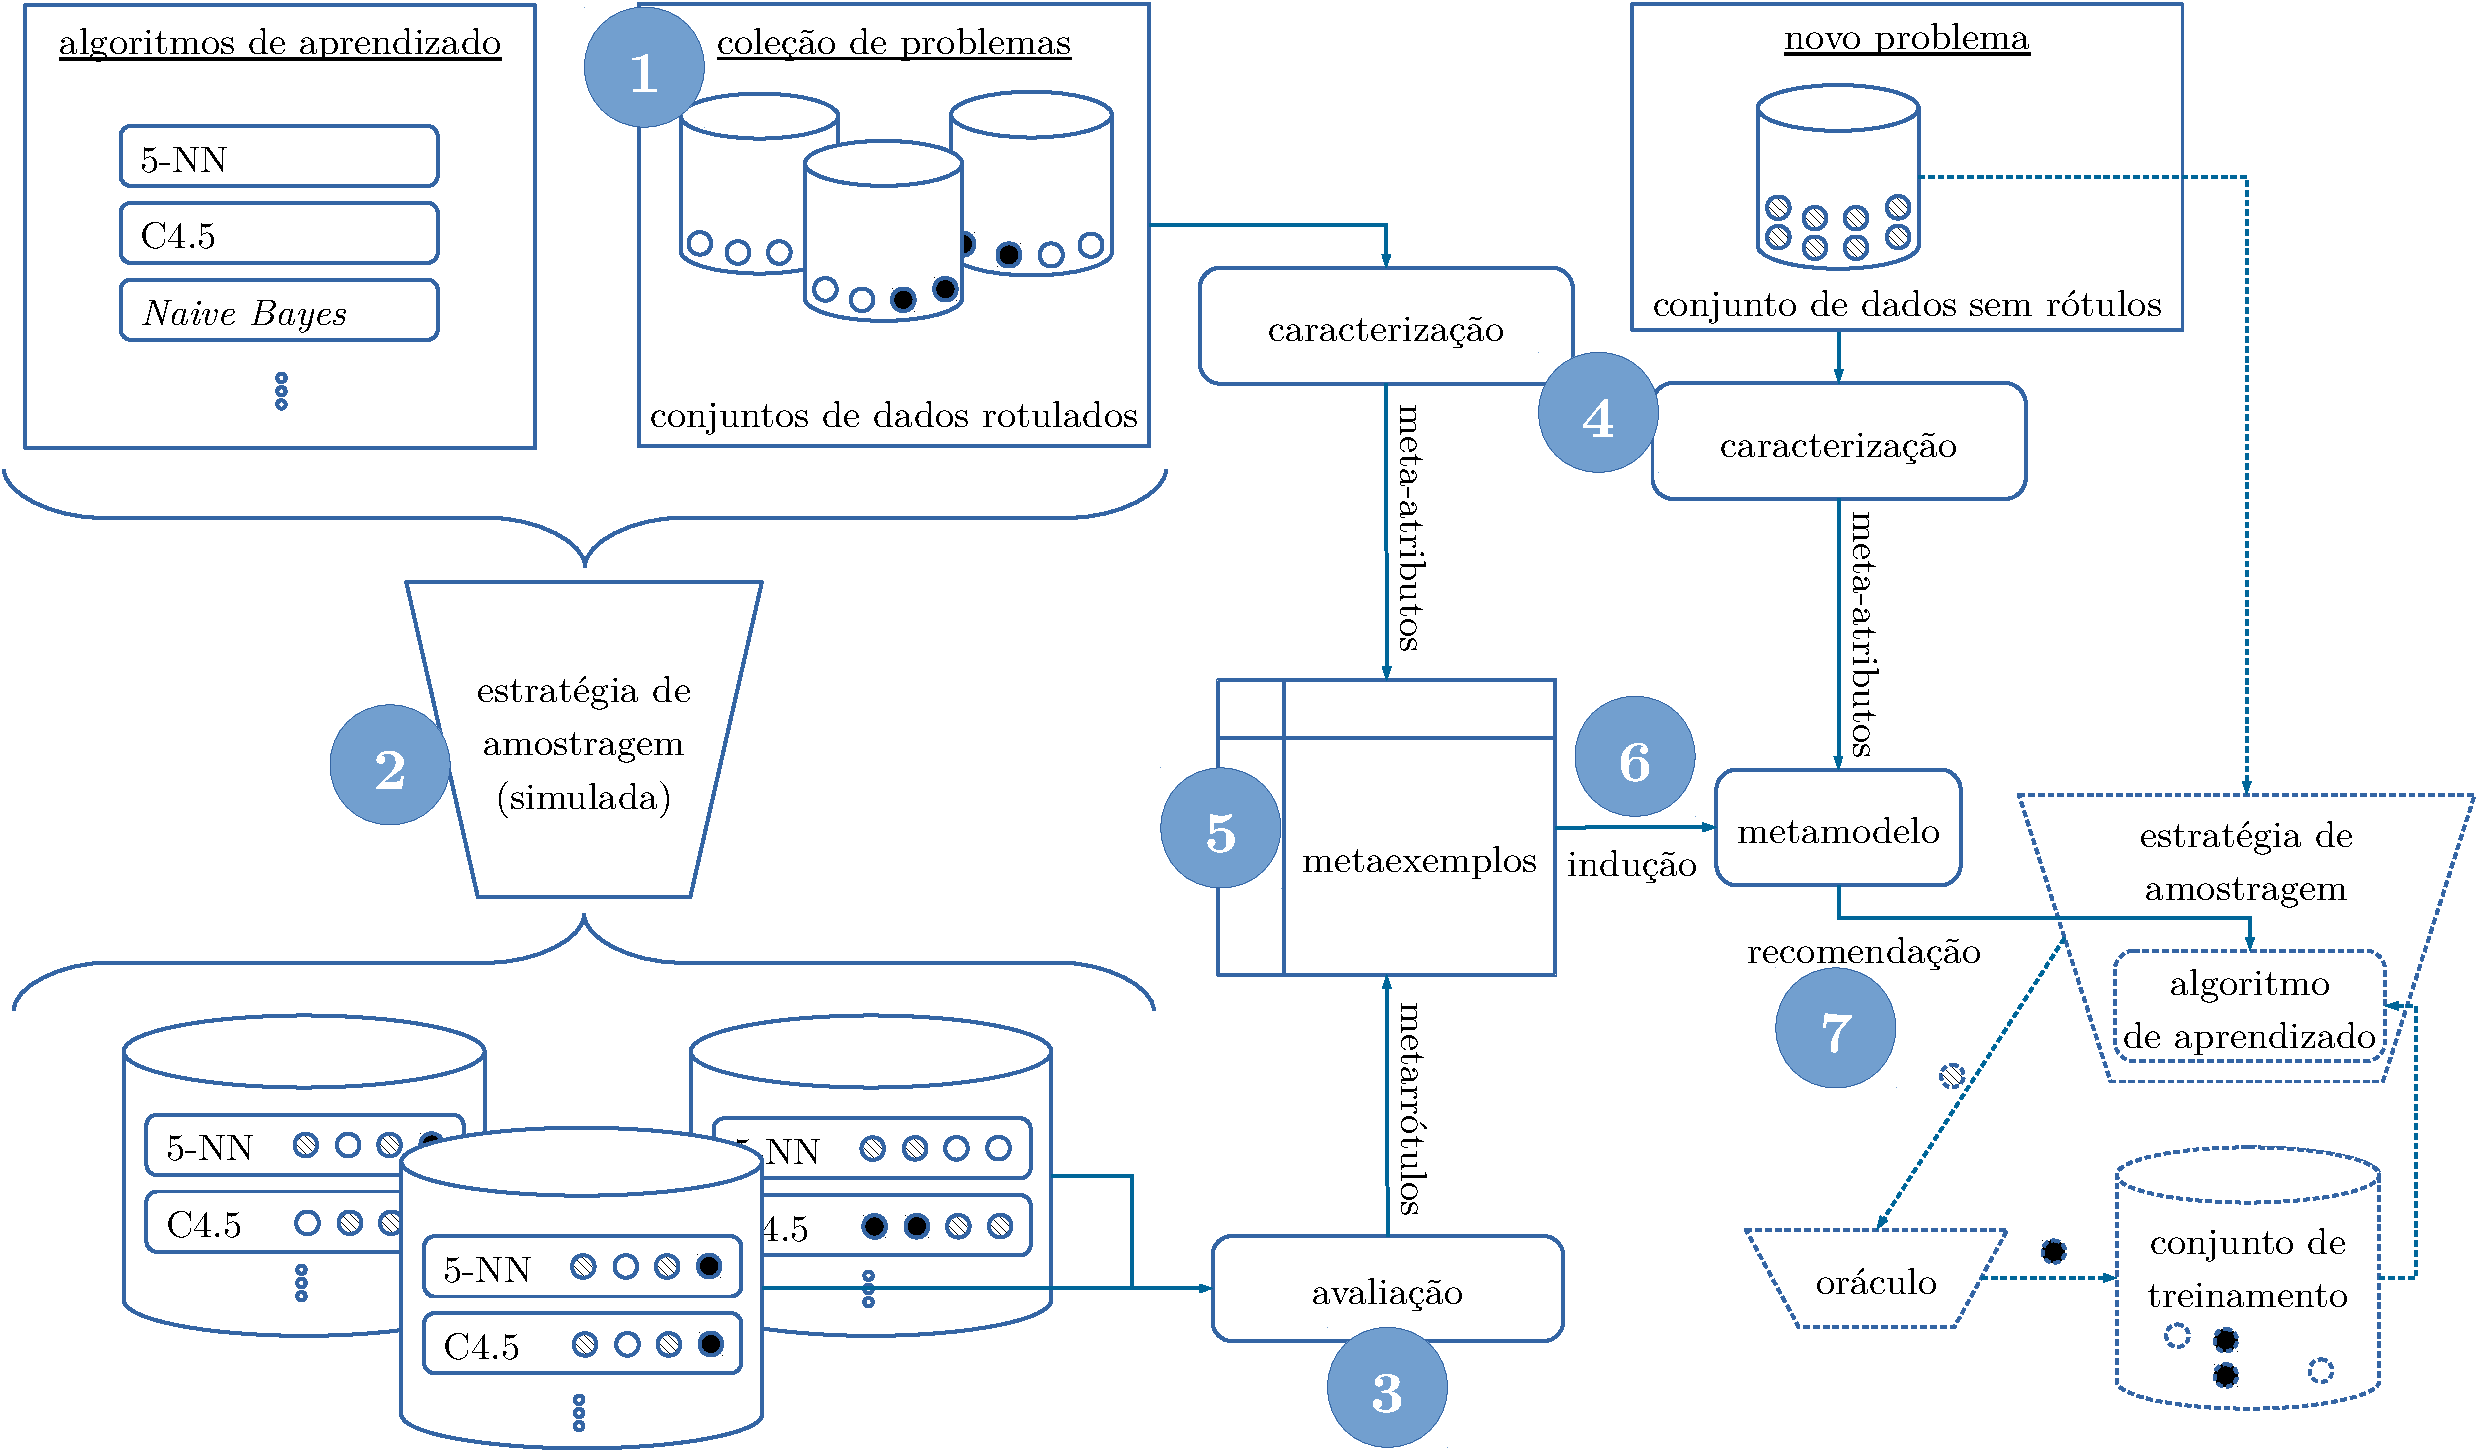
\includegraphics[scale=0.57]{images/meta.pdf}
	\caption[Esquema do sistema de recomendação.]{Esquema do sistema de recomendação. \textit{Os elementos tracejados representam o ciclo usual de aprendizado ativo, que aqui usufrui do meta-aprendizado. Nessa proposta inicial, a estratégia é sempre a mesma.}}
	\label{esquema}
\end{figure}
\end{landscape}

A obtenção de informações sobre o desempenho de estratégias em conjuntos já rotulados requer a caracterização destes (Passo \ref{passo4}).
A caracterização ocorre por meio da extração de medidas que descrevam os dados, chamadas \textit{meta-atributos}.
Uma vez caracterizados, os conjuntos tornam-se comparáveis entre si e viáveis para a construção de um metaconjunto de treinamento, pois passaram a ser representados num mesmo espaço de meta-atributos, como metaexemplos (Passo \ref{passo5}).
O metamodelo induzido com os metaexemplos (Passo \ref{passo6}) é, então, capaz de fazer recomendações de algoritmos (Passo \ref{passo7}) para a estratégia de amostragem ativa (não mais simulada).

Usualmente, medidas estatísticas simples, como \textit{assimetria} e \textit{curtose} são calculadas para cada atributo numérico do conjunto de dados.
Essas medidas estão presentes no STATLOG (Seção \ref{direta}), um dos primeiros sistemas de meta-aprendizado.
Ele contempla conjuntos de dados com diferentes quantidades de atributos numéricos, criando um meta-atributo para cada medida.
Assim, cada meta-atributo consiste na média dos valores da medida ao longo de todos os atributos numéricos.
Segundo \citeonline{kalousis2002algorithm}, essa abordagem por médias incorre em perda de poder discriminatório.
Sua alternativa foi a adoção de histogramas com a contagem de ocorrências em determinadas faixas de valores.
Nesta tese, devido à impossibilidade de prever o intervalo total de ocorrência dos valores e definir seu particionamento, optou-se por substituir o esquema de histogramas por um esquema limitado a alguns valores relevantes.
Esses valores seriam o mínimo, o máximo, o médio e a razão entre o mínimo e o máximo.
Na presente proposta, as medidas escolhidas para caracterização dos conjuntos foram obtidas de alguns trabalhos da literatura de meta-aprendizado.
As medidas são descritas no Quadro \ref{metats}.
\begin{quadro}
\simbolo{\qatt,\qexe,\qnc,\qexeatt,\pno,\lgqexe,\lgqexeatt,\qnom_{min},\qnom_{max},\qnom_{mea},\qnom_{min/max},{\mu}_{min},{\mu}_{max},{\mu}_{mea},{\mu}_{min/max}}{meta-atributos descritos no Quadro \ref{metats} (parte 1/4)}
\simbolo{\sigma_{min},\sigma_{max},\sigma_{mea},\sigma_{min/max},\en_{min},\en_{max},\en_{mea},\en_{min/max},\rho_{min},\rho_{max},\rho_{mea},\rho_{min/max}}{meta-atributos descritos no Quadro \ref{metats} (parte 2/4)}
\simbolo{\sk_{min},\sk_{max},\sk_{mea},\sk_{min/max},\ku_{min},\ku_{max},\ku_{mea},\ku_{min/max},\cn_{k1},\cn_{k1.5},\cn_{k2},\cn_{h1},\cn_{h1.5},\cn_{h2}}{meta-atributos descritos no Quadro \ref{metats} (parte 3/4)}
\simbolo{\du_{k1},\du_{k1.5},\du_{k2},\du_{h1},\du_{h1.5},\du_{h2},\si_{k1},\si_{k1.5},\si_{k2},\si_{h1},\si_{h1.5},\si_{h2}}{meta-atributos descritos no Quadro \ref{metats} (parte 4/4)}
\centering
% \renewcommand\tablename{Quadro}
\caption{Descrição dos 53 meta-atributos.}
\label{metats}
\begin{threeparttable}
\begin{tabular}{|p{3.6cm}|p{4.6cm}|m{6cm}|}
\hline
\textbf{Meta-atributo} & \textbf{Descrição}&\textbf{Fórmula} \\ \hline
$\qatt$ & número de atributos\tnote{a} & $|\mathcal{A}|$ \\ \hline
$\qexe$ & número de exemplos\tnote{a} & $|\mathcal{U}|$ \\ \hline

$\qnc$ & número de classes\tnote{b} & $|Y|$ \\ \hline

$\qexeatt$ & proporção de exemplos para atributos\tnote{c} &
$\frac{|\mathcal{U}|}{|\mathcal{A}|}$
\\ \hline

$\pno$ & proporção de atributos nominais\tnote{c} & 
$\frac{1}{|\mathcal{A}|}|\{A\in \mathcal{A} \mid \nom(A)=1\}|$ \\ \hline

$\lgqexe$ & logaritmo do número de exemplos\tnote{d} &
$\log|\mathcal{U}|$ \\ \hline

$\lgqexeatt$ & logaritmo da proporção exemplos/atributos\tnote{d} &
$\log\frac{|\mathcal{U}|}{|\mathcal{A}|}$ \\ \hline


$\qnom_{min}$, $\qnom_{max}$, $\qnom_{mea}$, $\qnom_{min/max}$ & 
qtd. de valores nominais:\tnote{c}\phantom{c} 
\textit{mínima, máxima, média e mín./máx. por atributo\tnote{c'}\phantom{c'}} &
$\qnom_{A} = |A|, A \in \mathcal{A}$ \\ \hline


${\mu}_{min}$, ${\mu}_{max}$, ${\mu}_{mea}$, ${\mu}_{min/max}$ &
média\tnote{c}\phantom{c} (\textit{idem}) & 
$\mu_j = \frac{1}{|\mathcal{U}|} \sum\limits_{\bm{x} \in \mathcal{U}} x_j$
$1 \leq j \leq |\mathcal{A}|$ \\ \hline

$\sigma_{min}$, $\sigma_{max}$, $\sigma_{mea}$, $\sigma_{min/max}$ &
desvio padrão\tnote{b}\phantom{b} (\textit{idem}) & 
$\sigma_j = \frac{1}{|\mathcal{U}|} \sum\limits_{\bm{x} \in \mathcal{U}}(x_j - \mu_j)^2$
\\ \hline

$\en_{min}$, $\en_{max}$, $\en_{mea}$, $\en_{min/max}$ &
entropia normalizada\tnote{b}\phantom{b} (\textit{idem}) & 
$\en_j = \frac{-1}{\log|\mathcal{U}|} \sum\limits_{\bm{x} \in \mathcal{U}} x_j\log x_j$
\\ \hline

% pearson
$\rho_{min}$, $\rho_{max}$, $\rho_{mea}$, $\rho_{min/max}$ &
correlação entre pares de atributos\tnote{b}\phantom{b} (\textit{idem}) & 
$\rho_{jk} = $ \phantom{ooooooooooo} \phantom{oooooooo}
$(\sigma_j^2\cdot\sigma_k^2)^{-\frac{1}{2}}
\sum\limits_{\bm{x} \in \mathcal{U}} 
(x_j - \mu_j)(x_k - \mu_k)$ \\ \hline

$\sk_{min}$, $\sk_{max}$, $\sk_{mea}$, $\sk_{min/max}$ &
assimetria\tnote{b}\phantom{b} (\textit{idem}) & 
$ \sk_j = \frac{n}{(n -1)(n - 2)} \sum\limits_{\bm{x} \in \mathcal{U}}
\frac{(x_j - \mu_J)^3}{\sigma_j^3}$
\\ \hline

$\ku_{min}$, $\ku_{max}$, $\ku_{mea}$, $\ku_{min/max}$ &
curtose\tnote{b}\phantom{b} (\textit{idem}) & 
\makecell{$\ku_j =  \frac{n(n+1)}{(n -1)(n - 2)(n-3)}
\sum\limits_{\bm{x} \in \mathcal{U}}
\frac{(x_i - \mu_j)^4}{\sigma_j^4}$\\
$- 3(n-1)^2[(n-2)(n-3)]^{-1}$} \\ \hline

% Internal evaluation
% dunn: compactação e separação; silhueta: ?
$\cn_{k1}$, \phantom{ll}$\cn_{k1.5}$, \phantom{ll}$\cn_{k2}$,
$\cn_{h1}$, \phantom{ll}$\cn_{h1.5}$, \phantom{ll}$\cn_{h2}$ &
conectiv.\tnote{e}\phantom{e} \textit{k-médias} \phantom{oooo}
conectiv \textit{agrup. hierárq.} & 
agrupam. \cite{xu2008clustering}
\textit{qtd. de grupos: $|Y|$; $1,5|Y|$ e $2|Y|$}\\
\hline

$\du_{k1}$, \phantom{l}$\du_{k1.5}$, \phantom{l}$\du_{k2}$,
$\du_{h1}$, \phantom{l}$\du_{h1.5}$, \phantom{l}$\du_{h2}$ &
índ. Dunn\tnote{e}\phantom{e} \textit{k-médias} \phantom{ooo}
índ. Dunn \textit{agr. hierárq.} &
agrupam. \cite{dunn1973fuzzy} \phantom{oooooo} (\textit{idem}) \\ \hline


$\si_{k1}$, \phantom{aa}$\si_{k1.5}$, \phantom{aa}$\si_{k2}$,
$\si_{h1}$, \phantom{aa}$\si_{h1.5}$, \phantom{aa}$\si_{h2}$ &
silhueta\tnote{e}\phantom{e} \textit{k-médias} \phantom{ooooo}
silhueta \textit{agrup. hierárq.} &
agrupam. \cite{rousseeuw1987silhouettes} (\textit{idem}) \\ \hline

\end{tabular}
\begin{tablenotes}
\item [a] Caracterização sugerida por \citeonline{conf/ijcai/RendellST87}.
\item [b] Baseado no projeto STATLOG \cite{brazdil1994analysis}.
\item [c] Baseado no conjunto de \citeonline{kalousis2002algorithm}.
\item [c'] Adaptação da sumarização proposta por \citeonline{kalousis2002algorithm}.
\item [d] Meta-atributos para recomendar algoritmos de agrupamento \cite{conf/ijcnn/SoutoPSACLS08}.
\item [e] Meta-atributos para recomendação de algoritmos de classificação \cite{souza2010meta}
e de algoritmos de agrupamento \cite{Ferrari2015181}.
\end{tablenotes}
\end{threeparttable}

\end{quadro}

\simbolo{\gamma}{metaclasse}
\simbolo{\chi}{metaexemplo}
\simbolo{\Lambda}{metaconjunto de dados}
\simbolo{\eta}{metamodelo}
\simbolo{\psi(\Lambda)}{função indutora para o metaconjunto de dados $\Lambda$}
Finalmente, o esquema proposto segue o Algoritmo \ref{algmta}.
O esquema é o mesmo nas demais formas de recomendação, com pequenas alterações triviais.
Na recomendação de estratégias, escolhe-se um algoritmo de antemão e, na recomendação de pares estratégia-algoritmo, ambos compõem a informação de metaclasse.
\begin{algoritmo}
\caption{Recomendação automática de algoritmos de aprendizado.}
  \small
\label{algmta}
\Entrada{
 \\ $\Phi$ - conjunto de funções indutoras $\phi$ (algoritmos)
 \\ $\mathfrak{L}$ - coleção de conjuntos de dados rotulados
 \\ $\psi$ - função de indução (algoritmo do meta-aprendiz)
 \\ $\cent$ - orçamento (50 ou 100 exemplos a rotular)
 \\ $q$ - função-critério que representa a estratégia (Algoritmo \ref{algo})
 \\ $k$ - número de partições da validação cruzada
 \\ $\mathcal{U}$ - novo conjunto de dados sem rótulos
}
\Resultado{
 \\ $\phi$ - função indutora recomendada (algoritmo do aprendiz ativo)
}
\algalg{\treina{$\Phi$, $\mathfrak{L}$, $\psi$, $\cent$, $q$, $k$, $\mathcal{U}$}}{
  $\Lambda\leftarrow\varnothing$\\
  \paracada {$\mathcal{L}\in\mathfrak{L}$}{    
    $\gamma=$ \best{$\Phi$, $\mathcal{L}$, $\cent$, $q$, $k$} \come{metaclasse}\\    
    $\bm{\chi} = (\qatt,\qexe,\qnc,\qexeatt,\pno,\lgqexe,\lgqexeatt,\qnom_{min},\qnom_{max},\qnom_{mea},\qnom_{min/max},$ 
    \phantom{$\bm{\chi}= ($}${\mu}_{min},{\mu}_{max},{\mu}_{mea},{\mu}_{min/max},\sigma_{min},\sigma_{max},\sigma_{mea},\sigma_{min/max},$
    \phantom{$\bm{\chi}= ($}$\en_{min},\en_{max},\en_{mea},\en_{min/max},\rho_{min},\rho_{max},\rho_{mea},\rho_{min/max},$
    \phantom{$\bm{\chi}= ($}$\sk_{min},\sk_{max},\sk_{mea},\sk_{min/max},\ku_{min},\ku_{max},\ku_{mea},\ku_{min/max},$
    \phantom{$\bm{\chi}= ($}$\cn_{k1},\cn_{k1.5},\cn_{k2},\cn_{h1},\cn_{h1.5},\cn_{h2},\du_{k1},\du_{k1.5},\du_{k2},\du_{h1},\du_{h1.5},\du_{h2},$
    \phantom{$\bm{\chi}= ($}$\si_{k1},\si_{k1.5},\si_{k2},\si_{h1},\si_{h1.5},\si_{h2})$ \come{meta-atributos extraídos de $\mathcal{L}$}\\
%     Usei parêntesis porque pode ser um vetor, já que todos os meta-atributos são numéricos.
    $\Lambda\leftarrow\Lambda\cup\{\langle \bm{\chi},\gamma\rangle\}$
  }
  $\eta\leftarrow\psi(\Lambda)$ \come{induz metamodelo} \\
  \Retorna $\eta$
}
\algalg{\recomenda{$\eta$, $\cent$, $\mathcal{U}$}}{
	$\bm{\chi}= (\qatt, ...,\si_{h2})$ \come{meta-atributos extraídos de $\mathcal{U}$}\\
	$\phi \leftarrow \hat{y}_{\eta}(\bm{\chi})$\\
  \Retorna $\phi$
}
\end{algoritmo}


% % 
% % ;
% % \ano{\cite{conf/ijcnn/SoutoPSACLS08}, sobre clustering,
% % ``melhoram`` statlog, aplicando log}
% 

\section{Considerações}
Neste capítulo, as estratégias ATU e HTU foram propostas juntamente com a adaptação SGmulti e o sistema de recomendação baseado em meta-aprendizado.
Todas as propostas foram textualmente e algoritmicamente descritas.
No Quadro \ref{strats}, as novas estratégias são incorporadas à lista comparativa de estratégias previamente descritas no Capítulo \ref{contexto}.
\begin{quadro}
\caption[Características de cada estratégia, incluindo propostas.]{Características de cada estratégia, incluindo estratégias propostas (em negrito).}
\label{strats}
\centering
\begin{threeparttable}
\begin{tabular}{|l|p{3cm}|p{2cm}|l|p{3.2cm}|}
\hline
\textbf{Estratégia}		& \textbf{Busca}		&\textbf{Aprendiz}  & \textbf{Dependência}		&\textbf{Complexidade}  \\ \hline
Rnd\tnote{a}			& {exploratória aleatória} 		& ausente			& nenhuma							&dispensa treinamento  \\ \hline
\textbf{ATU}\tnote{k}			&{exploratória}		& sem aprendiz				& nenhuma 							&dispensa treinamento  \\ \hline
HS\tnote{b}			&{balanceada exploratória prospectiva}	& ausente		& total							&dispensa treinamento\tnote{*}  \\ \hline
Mar/Ent\tnote{a} /QBC\tnote{c}	& prospectiva					& presente		& total							&$\mathcal{O}(1)$  \\ \hline
DW\tnote{d}			& prospectiva					& presente		& total							&$\mathcal{O}(1)$  \\ \hline
EER\tnote{e}			& prospectiva					& presente	& total							&$\mathcal{O}(|Y||\mathcal{U}|^2)$  \\ \hline
TU\tnote{f}			&{balanceada exploratória prospectiva}	& presente		& total							&$\mathcal{O}(1)$  \\ \hline
SGnetwork\tnote{g}		&{limitada exploratória aleatória}	& presente			& total							&$\mathcal{O}(1)$  \\ \hline
\textbf{SGmulti}\tnote{g}		&{limitada exploratória aleatória}	& presente			& total							&$\mathcal{O}(|Y|)$  \\ \hline
SVMsim\tnote{h}			& prospectiva					&{presente \phantom{oooo} específico}	& total							&$\mathcal{O}(|\mathcal{L}||\mathcal{U}|)$  \\ \hline
EGL\tnote{i}			& prospectiva					&{presente \phantom{oooo} específico}	& total							&$\mathcal{O}(|Y||\mathcal{U}|)$  \\ \hline
SVMbal\tnote{j}			&{combinada exploratória prospectiva}&{presente \phantom{oooo} específico}			& total							&$\mathcal{O}(|\mathcal{L}||\mathcal{U}|)$  \\ \hline
\textbf{HTU}\tnote{k}			&{combinada exploratória prospectiva}&{combinação \phantom{oo} ausente\phantom{oooo} presente}	&{total}			&$\mathcal{O}(1)$  \\ 
\hline
\end{tabular}
\begin{tablenotes}
\item [*] Na ausência de aprendiz não há treinamento, porém HS tem sua própria complexidade a ser considerada.
\item [a] Amostragem aleatória, por margem ou entropia \cite{series/synthesis/2012Settles}.
\item [b] Amostragem hierárquica \cite{journals/tcs/Dasgupta11}.
\item [c] Consulta por comitê \cite{conf/icml/AbeM98}.
\item [d] Amostragem ponderada por densidade \cite{settles2008curious}.
\item [e] Redução esperada do erro \cite{conf/ijcai/GuoG07}.
\item [f] Amostragem ponderada por densidade e utilidade de treinamento \cite{settles2010active,journals/coling/FujiiITT98}.
% \item [g] SGnetwork \cite{journals/ml/CohnAL94}.
\item [g] SGmulti \cite{conf/hais/SantosC14}.
\item [h] Margem simples \cite{journals/jmlr/TongK01}.
\item [i] Comprimento esperado do gradiente \cite{conf/nips/SettlesCR07}.
\item [j] Balanceamento exploração-prospecção \cite{conf/icdm/OsugiKS05}.
\item [k] Amostragem ponderada por densidade sem aprendiz e híbrida \cite{bracis15}.
\end{tablenotes}
\end{threeparttable}
\end{quadro}

Resumidamente, a estratégia ATU consiste na remoção total do aprendiz de TU.
HTU consiste na ativação do aprendiz somente nos momentos em que o modelo preditivo esteja suficientemente estável, a ponto de manter a correlação entre a medida de incerteza e a função-critério de TU acima de um elevado limiar. 
SGmulti apenas estende o conceito da abordagem original, mantendo uma reserva de exemplos artificiais para cada classe.

A tentativa de aprendizado meta-ativo é uma nova abordagem na área de aprendizado ativo - até onde alcança o conhecimento do autor.
Ela é baseada na recomendação automática de algoritmos de aprendizado.
Inicialmente, meta-atributos são extraídos do conjunto de dados, caracterizando-o.
Uma base de conhecimento previamente construída por meio da caracterização de outros conjuntos, cujos melhores algoritmos de aprendizado são conhecidos, é utilizada como metaconjunto.
Idealmente, um metamodelo induzido com esse metaconjunto permitiria predizer qual o melhor  algoritmo e, possivelmente, a melhor estratégia ou o melhor par estratégia-algoritmo.

As propostas aqui apresentadas foram avaliadas empiricamente de acordo com a metodologia descrita no Capítulo \ref{metodologia}.
